\section{Grundlagen}
\label{cha:grundlagen}
%Im Grundlagenkapitel stellen Sie das Basiswissen für die weiteren Kapitel vor.
%Hierzu können neben theoretischen Konzepten auch die historische Entwicklung
%und aktuelle Forschungsvorhaben gehören. Idealerweise bedient man sich hier
%mehrerer verschiedener Quellen, um die Ausführungen zu belegen.

%Nachfolgend werden einige Formalitäten der Arbeit dargestellt.


In dieser Arbeit soll für "`Independent Software Vendors"', also unabhängige
Softwarehersteller ein Vorgehensmodell für Cloud-Migrationen zu Salesforce
entwickelt werden. Aus diesem Ziel ergeben sich grundlegende Fragen, die in
diesem Kapitel beantwortet werden sollen:
\begin{itemize}
	\item Welche Vorteile bietet die Cloud und wie lassen sie sich
erzielen? Inwiefern unterscheiden sich Cloud-Migrationen von herkömmlichen
Migrationen in der IT und wie lassen sie sich zum Outsourcing abgrenzen? 
	\item Was wird in dieser Arbeit unter "`Independent Software Vendors"'
verstanden? Welche Besonderheiten weisen sie und ihre Projekte auf und welchen
Einfluss haben diese Besonderheiten auf Cloud-Migrationen?
	\item Warum ist Salesforce als Zielplattform für Migrationen
geeignet?
	\item Welche Faktoren beeinflussen die Cloud-Migration und ihren
Erfolg?
\end{itemize}
Das Kapitel wird von der Vorstellung des Fünf-Phasen-Modells abgeschlossen,
auf dem das entwickelte Vorgehensmodell basiert. Auch wird die Wahl für dieses
Modell als Arbeitsgrundlage begründet.

\subsection{Migration und Cloud-Migration}
\label{cha:definition_cloud-migration}

Die Migration von Software, wird in der Norm ISO/IEC 14764 "`Software
Engineering -- Software Life Cycle Processes -- Maintenance"' als spezielle
Form der Wartung, nämlich als anpassende Wartung ("`Adaptive Maintenance"') und
Weiterentwicklung definiert, bei der eine Software nach Auslieferung geändert
wird, um das Produkt in geänderten oder sich ändernden Umgebungen nutzbar zu
halten. \pcite{}{}{characterizing_software_architecture_changes} \\
Beispiel für eine solche Migration ist der Umzug einer Software auf neue
Hardware mit aktualisiertem Betriebssystem. Grund für den Umzug könnte ein
technischer sein, wie etwa dass keine Ersatzteile mehr für die vorhandene
Hardware angeboten werden, dass der Support des Herstellers für das laufende
Betriebssystem ausläuft. Aber auch wirtschaftliche Gründe, wie etwa eine
geforderte, höhere Leistungsfähigkeit oder ein geringerer Energieverbrauch des
neuen Systems sind denkbar. \\
Um die Software lauffähig zu halten, muss sie gegebenenfalls an das
aktualisierte Betriebssystem oder die Laufzeitumgebung angepasst werden.
Je standardisierter und verbreiteter die Anforderung der zu migrierenden
Software, desto geringer werden die nötigen Anpassungen an der
Software ausfallen, womit die Migration einfacher und kostengünstiger wird.
Eventuell wird lediglich eine virtuelle Maschine auf einen neuen Server
gestartet. 

Eine solche virtuelle Maschine ließe sich auch in der Cloud starten. Auf diese 
Weise ließen sich jedoch nicht die folgenden Vorteile realisieren, die 
\citeflow{exploring_the_factors} als Hauptgründe für eine Migration in die 
Cloud identifiziert haben:
\begin{description}
	\item[Kosteneinsparungen] Cloud-Anbieter, die große Rechenzentren
mit vielen Servern betreiben können die Total Cost of Ownership pro Server um
bis zu 80\% reduzieren (Vgl. Abbildung~\ref{fig:tco_reduction}).
\begin{figure}[!h]
\begin{center}
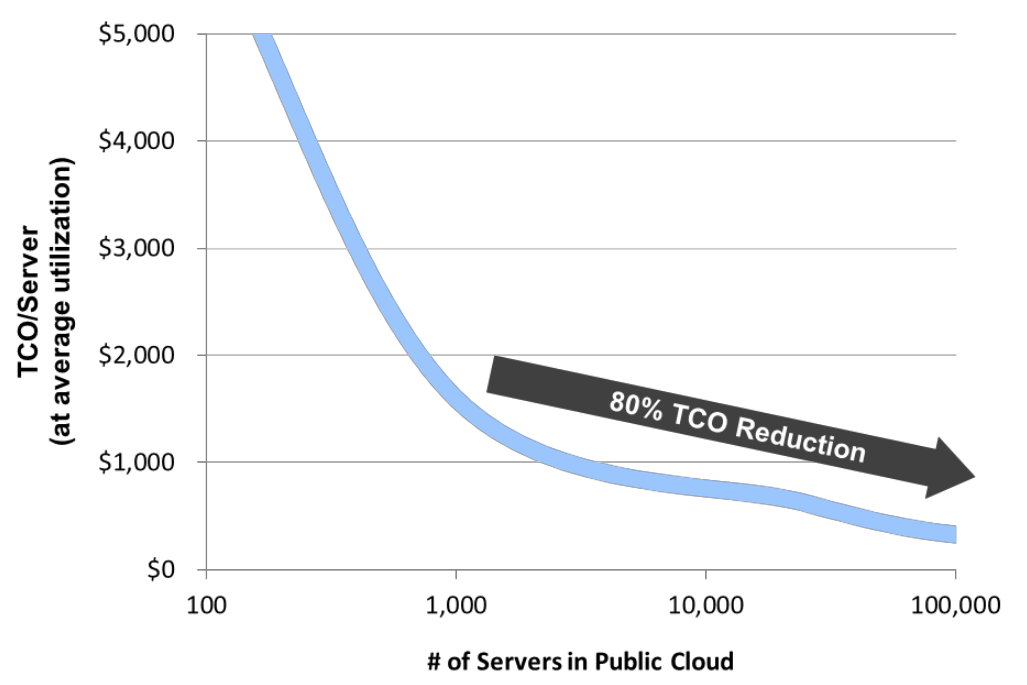
\includegraphics[width=0.8\textwidth]{images/tco_reduction.png}
\caption{Total Cost of Ownership/Server
aus \protect\citeflow{economics_of_the_cloud}}
\label{fig:tco_reduction}
\end{center}
\end{figure}
 Hauptsächlich geschieht dies über die Faktoren Energie-, Lohn- und
Hardwarekosten. Energiekosten lassen sich durch die Wahl eines Standortes
mit günstigem Strom niedrigen Umgebungstemperaturen senken. Durch
Automatisierungstechniken lässt sich die Zahl der Server, die ein Administrator
betreibt verzehnfachen, wodurch die Lohnkosten sinken. Hardwarekosten fallen
durch bessere Verhandlugspositionen großer Cloud-Anbieter niedriger aus.
\pcite{}{}{cloud_migration}

Die niedrigeren Kosten werden über den Markt teilweise an die Kunden weiter
gegeben, die die kapitalintensive Beschaffung der Hard- und Software sowie die
Vorhaltung eigener Personalressourcen zur Entwicklung und Wartung reduzieren
können. \pcite{}{}{Repschlaeger2010}

	\item[Effiziente Ressourcennutzung] In der konventionellen IT-Welt
werden geschätzte 80\% der Ressourcen dazu verwendet, bestehende Infrastruktur
und Dienstleistungen zu betreiben, wodurch wenig Kapazität für wertstiftende
Tätigkeiten, wie die Entwicklung neuer Geschäftsfelder oder die Umsetzung von
Kundenwünschen bleibt. Cloud-Nutzung kann
dieses Verhältnis der Innovation verschieben. \pcite{}{}{economics_of_the_cloud}

	\item[Automatisierte, schnelle und unbegrenzte Skalierbarkeit der
Ressourcen] Die Zuteilung zusätzlicher, auf den Kunden unbegrenzt wirkender
Rechenleistung erfolgt in der Cloud entweder über ein einfaches Webformular oder
ausgerichtet am momentanen Bedarf voll automatisch. Da der Kunde nur das
bezahlen muss, was er benötigt, ist die Cloud gerade für Start-ups, kleine und
mittlere Unternehmen, sowie Unternehmen interessant, die entweder einen stark
schwankenden oder nicht abschätzbaren Bedarf haben; die Gefahr zu viel
Rechenleistung vorzuhalten, was zu unnötig hohen Kosten führt oder zu wenig
Rechenleistung, was Kunden abschrecken könnte,
sinkt.
\pcite{}{}{
economics_of_the_cloud, a_holistic_model_for_making_cloud_migration_decision,
migrating_to_the_cloud_lessons_and_limitations}

Das schnelle Deployment in der Cloud ermöglicht es, neue Ideen sehr
schnell zu implementieren, zu testen (falls gewünscht sogar im Vergleich zu
anderen Lösungen) und auszuwerten. Dadurch kann die Innovationsgeschwindigkeit,
Flexibilität und die "`Time to Market"' beachtlich gesteigert werden.
\pcite{}{}{factors_in_development_and_adoption,
decision-making_in_cloud_computing_environments, cloud_migration}

	\item[Geringerer Wartungsaufwand] Die Cloud treibt die Standardisierung
von Schnittstellen voran, sodass bestehende Funktionalitäten leichter
wiederverwendet werden können. Dadurch wird die Weiterentwicklung und Wartung
von Software reduziert. \pcite{}{}{economics_of_the_cloud}
\end{description}

\begin{comment}
Um von diesen Vorteilen profitieren zu können müssen 
die Software selbst, sowie Arbeitsprozesse und Geschäftsmodell angepasst 
werden. Da Umfang der Änderungen nicht mehr unter die oben genannte 
"`Weiterentwicklung"' fällt, wird von Cloud-Migrationen als Abgrenzung zu 
herkömmlichen Migrationen gesprochen. 
\pcite{}{}{framework_for_architecture-driven_migration}
\end{comment}


Der Grad, in dem diese Vorteile realisiert werden, davon ab, 
in welchem Umfang Leistungen in der Cloud in Anspruch genommen werden, was 
wiederum Einfluss auf den Migrationsprozess hat. \pcite{}{213}{Pahl2013}Zur 
Kategorisierung des Leistungsumfangs dienen "`as a Service"'-Modelle. Es
gibt recht viele dieser Modelle - \citeflow{xAsAService} zählt 35
Varianten - die mehr oder weniger verbreitet sind und mit "`Everything as a
Service"', abgekürzt als EaaS oder XaaS zusammengefasst werden. Dabei werden
nicht nur Technologien als Dienstleistung angeboten, sondern auch Ziele; so gibt
es beispielsweise auch "`Hardware-as-a-Service (HaaS)"' und
"`Business-Process-as-a-Service (BPaaS)"'.
\pcite{}{}{emerging_paradigms_and_areas_for_expansion, benlian_saas_2010}
\begin{figure}%[h]
\begin{center}
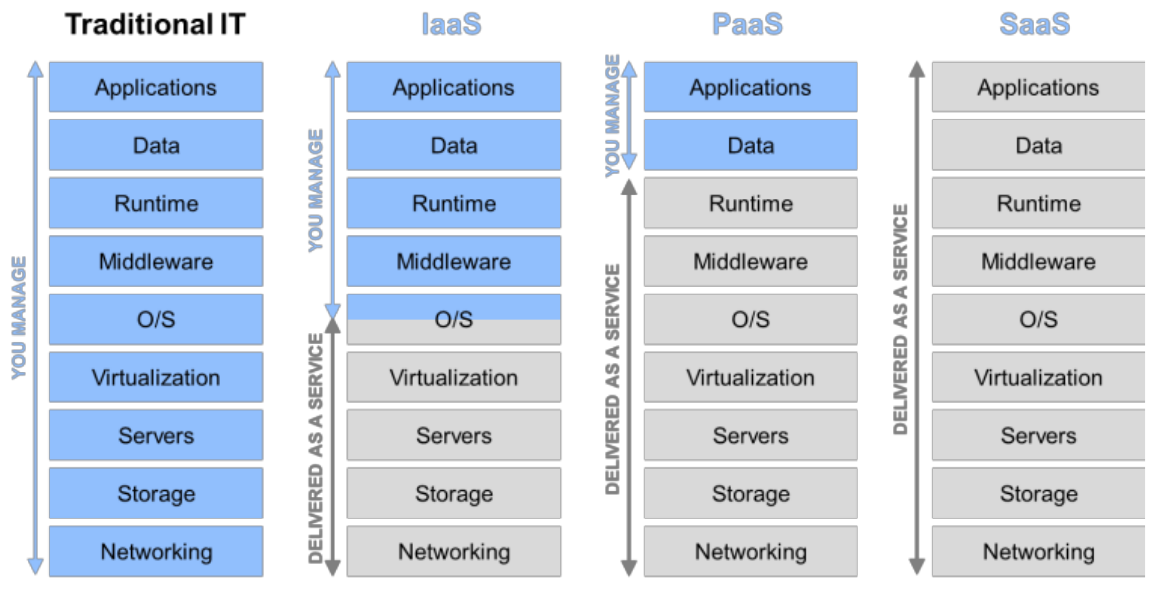
\includegraphics[width=\textwidth]{images/XaaS_im_Vergleich.png}
\caption{XaaS im Vergleich: Umfang von
Dienstleistung und Eigenverantwortung. Aus
\protect\citeflow{economics_of_the_cloud} }
\label{fig:xaas_im_vergleich}
\end{center}
\end{figure}

Das National Institute of Standards and Technology sieht drei
Service Modelle anerkannte vor, die sich im Anteil der
selbst zu verwaltenden, technologischen Anteile (Integrationstiefe)
unterscheiden und in dieser Hinsicht in Abbildung~\ref{fig:xaas_im_vergleich}
mit der herkömmlichen IT verglichen werden. \pcite{}{}{NIST,thoughtsOnCloud} 
\begin{description}
	\item[Infrastructure as a Service (IaaS)] Dem Kunden werden Netzwerk,
Speicher und Rechenleistung zur Verfügung gestellt. Über die darauf laufende
Software, teilweise sogar über das Betriebssystem kann selbst verfügt werden. \\
Kunden versprechen sich von IaaS vor allem Flexibilität in der Bereitstellung
und dem Betrieb von Servern, Datenspeichern und Netzwerkressourcen.
\pcite{}{213}{Pahl2013}
	\item[Platform as a Service (PaaS)] Der Kunde kann bereitgestellte
oder selbst entwickelte Software in der Cloud laufen lassen und eventuell
Einfluss auf die Anwendungsumgebung nehmen. 
	\item[Software as a Service (SaaS)] Der Kunde kann eine vom Anbieter
bereitgestellte Software nutzen und in begrenztem Maße konfigurieren.
\end{description}

Das für die Migration genannte Beispiel, eine virtuelle Maschine zu
verschieben, lässt sich mit Abbildung~\ref{fig:xaas_im_vergleich} für den
Cloud-Fall dem Modell IaaS zuordnen. Der Cloud-Kunde muss sich in diesem Fall
neben der eigentlichen Anwendung nach wie vor um das virtualisierte
Betriebssystem, Middleware, Laufzeitumgebung und Datenhaltung kümmern. Um die
Vorteile der Cloud besser auszuschöpfen, müsste die Anwendung entweder so
angepasst werden, dass sie auf einer zur Verfügung gestellten, fremdverwalteten
Laufzeitumgebung läuft (PaaS). Oder es wird eine bestehende Anwendung in der
Cloud genutzt und gegebenenfalls angepasst (SaaS). Beide Optimierungen
machen das Treffen konsequenzenreicher, kritischer Entscheidungen nötig, die 
nicht nur technische, sondern auch betriebswirtschaftliche und 
strategische Aspekte betreffen. \pcite{}{}{migration_to_paas_clouds}
Aus diesem Grund ist eine Cloud-Migration\footnote{Der Vollständigkeit halber
eine formale Definition der Cloud-Migration: "`Prozess der anteiligen
oder
vollständigen Bereitstellung von digitalen Gütern, Dienstleistungen,
IT-Ressourcen oder Anwendungen in der Cloud"'}
\pcite{}{}{Pahl2013} in ihrem Umfang viel mehr als eine Weiterentwicklung 
herkömmlicher Migrationen und erfordert eine dementsprechende, viel 
umfangreichere
Planung. \pcite{}{}{framework_for_architecture-driven_migration,
a_review_of_the_current_level_of_support_to_aid_decisions_for_migrating}

Für die zu migrierende Software gibt es zahlreiche Namen, zum Beispiel 
"`Software as a Product"' (SaaP) 
\pcite{}{}{changes_in_requirements_engineering}, "`Software as a Good"' 
\pcite{}{}{transitioning_to_saas} oder "`Legacy System"' 
\pcite{}{}{framework_for_architecture-driven_migration}. In dieser Arbeit wird 
der Begriff "`On-Premise-Software"' verwendet.

Der Ablauf von Cloud-Migrationen lässt sich in die folgenden Kategorien 
unterteilen: \citeflow{exploring_the_factors} 
\begin{description}
	\item[Ersetzen] Einzelne Komponenten einer bestehenden Anwendung werden
durch Dienste in der Cloud ersetzt. Andere Komponenten, die mit diesen
ersetzten Komponenten interagieren werden umkonfiguriert. Buzzwörter zu dieser 
Kategorie sind "`Service Oriented Architecture"' (SOA) und "`Microservices"': 
Anstatt Anwendungen als Monolithen gewaltigen Umfangs zu entwerfen, werden sie 
aus wiederverwertbaren Diensten konstruiert, die über Schnittstellen 
verbunden werden.
	\item[Partielle Migration] Anstatt Komponenten durch Cloud-Dienste zu
ersetzen, werden sie in die Cloud migriert.
	\item[Migration der ganzen Anwendung] Diesem Typus entspricht das 
Beispiel von oben: Eine Anwendung wird in ihrer virtuellen Maschine in die 
Cloud umgezogen.
	\item[Cloudify] Die Anwendung wird in Gänze an die Cloud und ihre
Charakteristika angepasst und mit Cloud Diensten neu entwickelt. Dieser Maxime 
folgt das in dieser Arbeit vorgestellte Modell.
\end{description}

%\subsubsection{Abgrenzung zum Outsourcing}

\subsection{Softwarehersteller: Independent Software Vendor (ISV)}
\label{cha:isv}
Unter dem Begriff "`Independent Software Vendor"' werden Softwarehersteller 
zusammengefasst, die Software für von ihnen unabhängige Plattformen, zum 
Beispiel Microsoft Windows oder Salesforce entwickeln.

\begin{figure}[!h]
\begin{center}
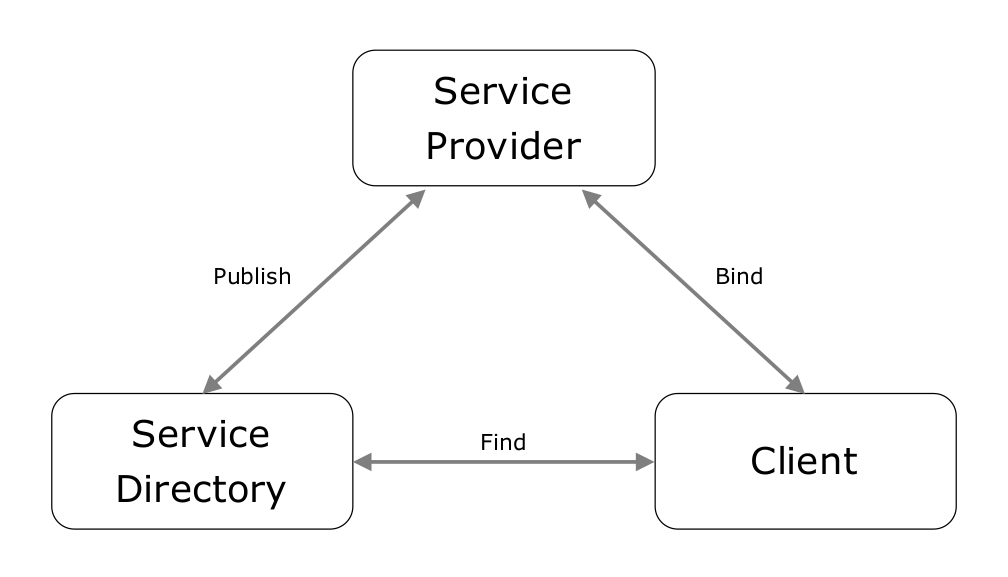
\includegraphics[width=0.8\textwidth]{images/soa_architecture.png}
\caption{Service-oriented architecture. Aus 
\protect\citeflow{changes_in_requirements_engineering}}
\label{fig:soa_architecture}
\end{center}
\end{figure}

\subsection{TODO: Synonyme für ISV}
Aus NIST cloud computing reference architecture "`Cloud Carrier"', 
"`Cloud Service Partner"' oder "`Cloud Service Developer"' (die letzten beiden 
aus \pcite{}{}{a_survey_and_taxonomy_of_cloud_migration})


Aus \citeflow{how_saas_changes_an_isvs_business}
\subsubsection{Vorteile für ISV}
\begin{itemize}
	\item Der Cloud-Markt ist größer und hat das Potential neue Kunden zu
erreichen, zum Beispiel kleinere Unternehmen für die eine Cloud-Lösung
günstiger ist oder Kunden in geographisch großer Distanz.
	\item Lösungen können direkt an Manager verkauft werden; Verhandlungen
mit den IT Abteilungen des Kunden werden minimiert. Inkompatibilitäten in Hard-
und Software beim Kunden werden vermieden.
	\item Monatliche oder jährliche Lizenzierungsgebühren stellen einen
kontinuierlicheren Umsatzstrom dar als Kaufverträge.
	\item Anstatt Support für viele Instanzen in unterschiedlichen
Umgebungen bei Kunden muss nur noch Support für die Cloud-Anwendung
geleistet werden.
	\item Da sich alle Kunden in der Cloud bewegen, weiß der ISV viel mehr
über sie und ihre Nutzungsart.
\end{itemize}

\subsubsection{Risiken für ISV}
\begin{itemize}
	\item Der Wechsel in der Cloud erfordert viele neue Ansätze, zum
Beispiel bei der Lizenzierung oder dem Verkauf und stellt einen großen Umbruch
dar.
	\item Da der Kunde die Cloud-Lösung in der Regel vor
Vertragsabschluss ausprobieren kann, muss der Anbieter einen echten Wert
bieten.
	\item Umsätze kommen zwar stetig aber in viel geringerer Höhe als bei
einem Kauf.
	\item Durch die Standardisierung bei SaaS kann die Anpassbarkeit
der Softwarelösung leiden.
\end{itemize}

\subsubsection{Auswirkungen auf das Geschäft durch SaaS}
Aus \citeflow{how_saas_changes_an_isvs_business}
\begin{description}
	\item[Markt] Das Angebot einer SaaS-Lösung könnte darauf abzielen,
bestehende Kunden und Märkte besser zu erreichen; möglicherweise unter
Kannibalisierung des bestehenden On-Premise-Produktes. Ziel könnte aber auch
sein, neue Märkte zu erschließen. Beide Ziele sind nicht exklusiv. Es ist
jedoch wichtig, sich der Möglichkeit der Schwerpunktbildung in dieser Frage
bewusst zu sein.
	\item[Preisgestaltung] Die meisten Preismodelle für SaaS-Anwendungen
haben eines der drei folgenden Modelle als Grundlage:
	\begin{itemize}
		\item Abonnement -- Nutzer pro Monat oder Gerät pro Jahr. Dies
ist das verbreitetste Modell. Durch Vergünstigungen bei Vorauszahlung für einen
längeren Zeitraum, können früh höhere Umsätze generiert werden.
		\item Pro Einheit -- Zahlung für jede Transaktion, jedes
gespeichertes/übertragenes Gigabyte oder für eine andere messbare Einheit, die
einen Nutzungsumfang beschreibt
		\item Free(mium) -- Das Basisprodukt ist kostenlos nutzbar oder
wird durch Werbeeinblendungen finanziert; Premiumfunktionen müssen bezahlt
werden
	\end{itemize}
	Die Wahl der Preisgestaltung hat bedeutenden Einfluss auf den Cashflow
des Unternehmens und ist in
Abbildung~\ref{fig:vergleich_umsatz_on-premise_cloud} dargestellt. Gerade die
Anfangsinvestition ist bei SaaS-Anwendungen häufig größer als bei
On-Premise-Anwendungen, gerade wenn das Unternehmen noch keine Erfahrungen mit
der Umsetzung hat. Diese Anfangsinvestition müssen ISV häufig leisten, bevor
Kunden akquiriert wurden. \\
Der Einfluss, den die Höhe des Preises auf das Geschäft hat, ist in
Abbildung~\ref{fig:einfluss_des_preises_auf_business} dargestellt. Bei der
Umstellung auf SaaS sollte darauf geachtet werden, dass Preis und die
Ausprägungen der anderen Aspekte in der gleichen Zeile liegen. So wird es sich
in der Regel für eine sehr günstige Anwendung nicht lohnen, einen externen
Verkaufsdienst in Anspruch zu nehmen oder eine persönliche Kundenbetreuung zu
garantieren. \\


\begin{figure}%[h]
\begin{center}
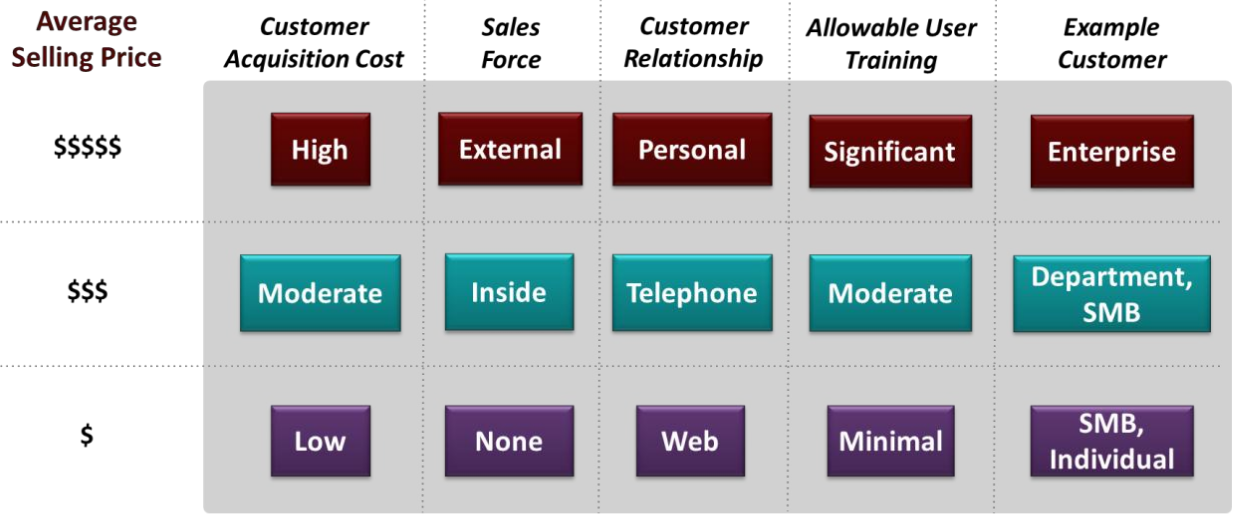
\includegraphics[width=\textwidth]{images/einfluss_des_preises_auf_business.png}
\caption{Der Einfluss des Preises auf das Geschäft. Aus
\protect\citeflow{how_saas_changes_an_isvs_business} }
\label{fig:einfluss_des_preises_auf_business}
\end{center}
\end{figure}

\begin{figure}%[h]
\begin{center}
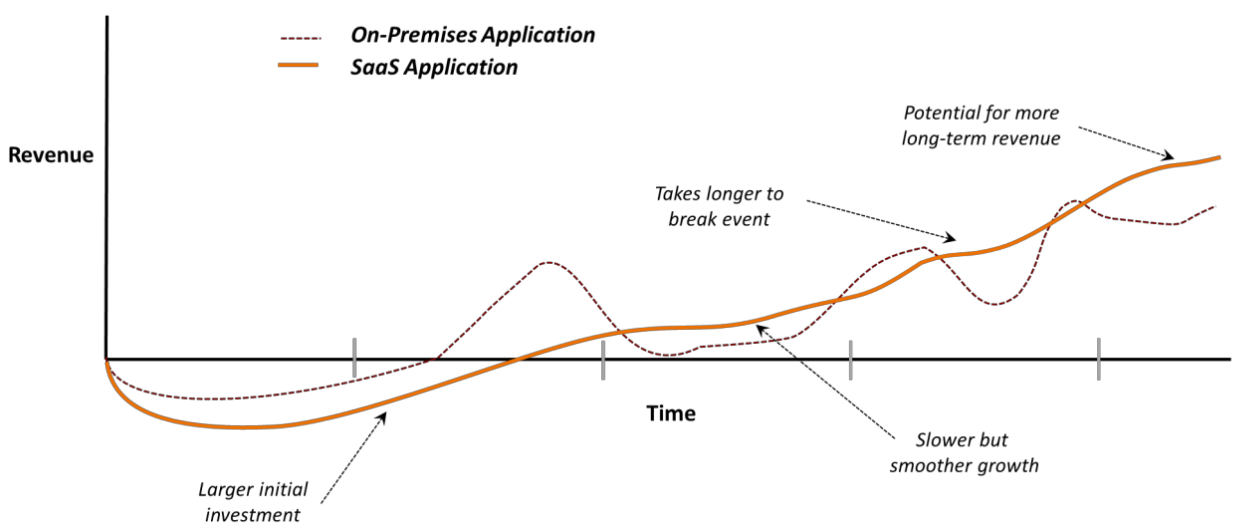
\includegraphics[width=\textwidth]{images/vergleich_umsatz_on-premise_cloud.png}
\caption{Die Umsätze von On-Premise-Anwendungen im Vergleich zu SaaS-
Anwendungen. Aus
\protect\citeflow{how_saas_changes_an_isvs_business} }
\label{fig:vergleich_umsatz_on-premise_cloud}
\end{center}
\end{figure}

	\item[Verkauf] Bei On-Premise-Anwendungen kann der Kunde die Anwendung
häufig erst nach dem Kauf in seiner Unternehmensumgebung testen und damit den
wahren Produktwert festellen, weil die Inbetriebnahme für Tests vor dem Kauf zu
aufwändig wäre. Bei SaaS-Anwendungen ist ein ausführliches Testen schon vor
Abschluss eines großen Lizenzvertrages möglich. Für den ISV kann dies ein
Vorteil sein, da die Einstiegshürden für Kunden vermindert sind: Mögliche
Fehlinvestitionen lassen sich reduzieren oder vermeiden, weshalb
Nutzungsentscheidungen vom Kunden von einer kleineren Gruppe von Managern
getroffen werden können. Ist das Produkt im Unternehmen, lassen sich benötigte
oder gewünschte Features leichter ermitteln. Der Kunde erhält ein Produkt nach
seinen Wünschen, der ISV Projektverträge um die Anwendung anzupassen oder
weiterzuentwickeln. Dieser Ansatz wird als "`land and expand"' bezeichnet.

\end{description}

\subsubsection{Entwicklung}
Da SaaS-Anwendungen werden typischerweise sehr viel häufiger geupdatet, als
On-Premise-Anwendungen. \pcite{}{}{how_saas_changes_an_isvs_business}

Die hohe Updatefrequenz macht agile Entwicklungsmodelle erforderlich, zum
Beispiel DevOps. \pcite{}{}{how_saas_changes_an_isvs_business}

\subsubsection{Organisationsstrukturen}
Was die Unternehmensstruktur angeht, gibt es für ISV, die ins SaaS-Geschäft
einsteigen wollen, drei Optionen, die in
Abbildung~\ref{fig:organisationsstrukturen} dargestellt sind.
\pcite{}{}{how_saas_changes_an_isvs_business}
\begin{enumerate}
	\item SaaS-Anwendungen entwickeln, ohne die bestehende
Unternehmensstruktur anzupassen hält den organisatorischen Aufwand zunächst
gering. Sollte das bestehende On-Premise-Geschäft weiterbetrieben werden, ist
es allerdings aufgrund der genannten Unterschiede zwischen den Modellen
schwierig, beides gut zu machen.
	\item Um dieses Problem zu lösen, kann eine Gruppe im Unternehmen
gegründet werden, dass sich ausschließlich mit dem Thema SaaS befasst.
	\item Manche Firmen lagern ihre SaaS-Bemühungen in eine wirtschaftlich
selbstständige Einheit aus. Dieser Ansatz erfordert unter Umständen die größten
strukturellen Änderungen, weil mit dem neuen Unternehmen erheblicher
Verwaltungsoverhead (Personalmanagement, Buchhaltung, etc.) einhergeht.
\end{enumerate}

\begin{figure}%[h]
\begin{center}
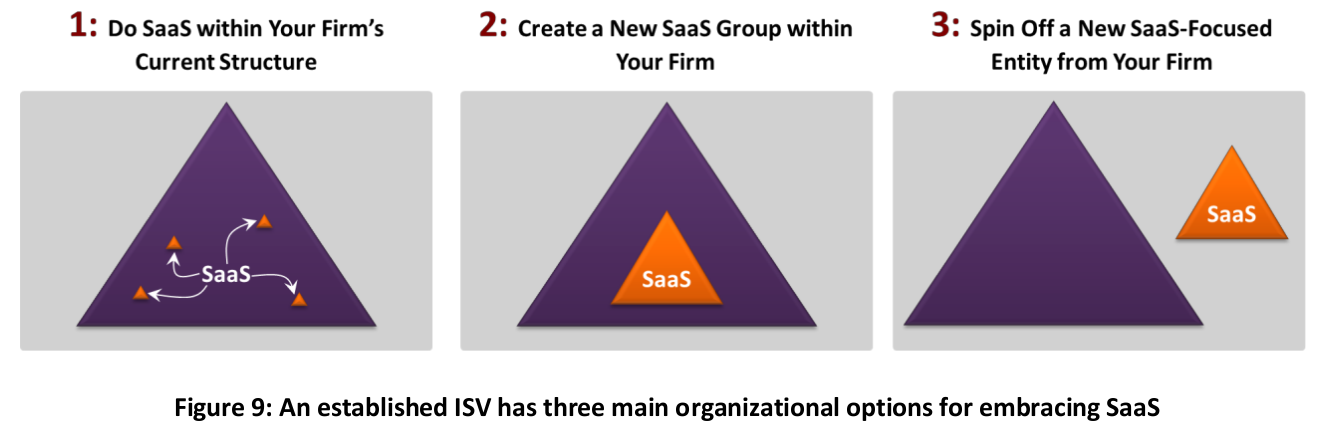
\includegraphics[width=\textwidth]{images/organisationsstrukturen.png}
\caption{Organisationsstrukturelle SaaS-Umsetzungsmöglichkeiten für ISV. Aus
\protect\citeflow{how_saas_changes_an_isvs_business} }
\label{fig:organisationsstrukturen}
\end{center}
\end{figure}

\subsubsection{Wahl des Cloud-Anbieters}
\citeflow{how_saas_changes_an_isvs_business} identifiziert vier Faktoren, die
bei der Entscheidung für einen CLoud-Anbieter zur Realisierung einer
SaaS-Anwendung berücksichtigt werden sollten:
\begin{description}
	\item[Anbietergröße] Wie in Kapitel~\ref{cha:vorteile_der_cloud}
geschildert, haben große Cloud-Anbieter Vorteile gegenüber kleinen. Vorhandene
Beziehungen und persönlichere Betreuung könnten dennoch für einen kleineren
Anbieter sprechen.
	\item[Geografische Verteilung] Um die Antwortzeiten für Kunden bei
Benutzung der SaaS-Anwendung niedrig zu halten, sollten Serverzentren
geografisch nah liegen. Entsprechend sollte ein weltweit agierender
Cloud-Provider gewählt werden, wenn ein weltweiter Markt adressiert werden
soll. Auch die Sicherheit vor Katastrophen spricht für eine möglichst breite
Verteilung.
	\item[Zuverlässigkeit] Mangelnde Zuverlässigkeit des Cloud-Providers
wird auf den ISV zurückfallen, weshalb ein in Backup-Mechanismen erfahrener
Provider gewählt werden sollte. Auch hier kann geografische Streuung ein
positiver Einflussfaktor sein.
	\item[Regulatorische Vorschriften] Gesetzliche Vorgaben können
erforderlich machen, dass der Cloud-Provider Nachweise über ihre Einhaltung
führt oder sogar, dass Daten in einem bestimmten Land gehalten werden. Nicht
alle Anbieter können dies leisten.
\end{description}


Die Änderungen, die SaaS für das Geschäft bringt überwiegen die
technischen. Da Änderungen aber
sowieso erforderlich sind, um auf
dem Markt zu bestehen, gibt es aber
eigentlich keine Wahl. \pcite{}{}{how_saas_changes_an_isvs_business}

Weil der Umstieg auf die Cloud nicht nur ein technisches Umdenken erforderlich
macht, sondern auch ein wirtschaftliches spricht
\citeflow{how_saas_changes_an_isvs_business} von einem ganz neuen Anbieter, dem
Cloud Service Vendors (CSV) anstatt ISV.
\pcite{}{3}{how_saas_changes_an_isvs_business}

\subsection{TODO: Devops als Entwicklungsmodell?}

\subsection{Salesforce als Zielplattform}
\label{cha:salesforce_als_zielplattform}
"`Die Ergebnisse belegen: Sämtliche Unternehmen konnten mit Force.com
hinsichtlich Entwicklungszeit und Supportkosten wesentliche Einsparungen
verzeichnen. Die Entwicklung mit Force.com war 4,9-mal schneller als mit JAVA
oder .NET"' \pcite{}{120}{benlian_saas_2010}

Customer Relationship Management (CRM) hat das Ziel Kunden zu gewinnen und zu
halten  und kombiniert dafür die Themen Prozesse, Menschen und Technologie als
übergeordnete Strategie, bei der es darum geht möglichst viel über den Kunden
zu erfahren. Salesforce kommt standardmäßig mit CRM.

Force.com ist eine etablierte Plattform um Cloud-Anwendungen zu entwickeln, zu
vertreiben und bei einer Verfügbarkeit von 99,9\% zu betreiben.
\pcite{}{}{a_new_way_of_developing}


\subsection{TODO: Faktoren übernehmen}
Aus \citeflow{cloud_adoption_decisions}

\subsection{Die Migration bestimmende Faktoren}
\label{cha:migration_bestimmende_faktoren}
\citeflow{fivephases} identifizieren wirtschaftliche und technische Faktoren,
die sowohl die Migrationseignung einer Anwendung als auch die Migration selbst
beeinflussen. \\
\citeflow{decision-making_in_cloud_computing_environments} sehen viele
Parallelen zwischen dem Outsourcen von IT zu externen
Dienstleistern und dem Betrieb in der Cloud, weshalb sich Erfahrungen bei
Outsourcing-Projekten bei Cloud-Migrationen
anwenden lassen. Aus diesem Grund sind die folgenden Faktoren auch aus der
Literatur über IT-Outsourcing zusammengetragen.
\subsubsection{Wirtschaftliche Faktoren}
\begin{description}
	\item[Bereits getätigte IT-Investitionen:]
	In der Regel wachsen die bereits getätigten IT-Ausgaben mit dem
Unternehmen und mit ihnen die Komplexität der Migration. Deshalb ist es in
kleinen Unternehmen eher möglich, direkt zu migrieren, während bei
größeren Unternehmen der Übergang in die Cloud wesentlich mehr Planung und
gegebenenfalls einen parallelen Betrieb erforderlich macht.

	\item[Kosten:] In der herkömmlichen IT bestehen Kosten aus der
"`kapitalintensiven Beschaffung der Hard- und Software sowie der Vorhaltung
eigener Personalressourcen"' \pcite{}{}{Repschlaeger2010}. Diese Kosten sind
zwar hoch, aber aufgrund der langjährigen Erfahrung auch vorhersagbar und in
Budgets eingeplant. Die Migration in die Cloud dagegen bedeutet den Umstieg zu
einem "`pay per use"'-Modell \pcite{}{}{elements_of_cloud_adoption}, von einem
von Fixkosten dominierten Modell zu einem, das von variablen Kosten bestimmt
ist.
Um zu verhindern, dass Kosteneinsparungen aufgezehrt werden, ist es nötig
den Umfang der Anwendungsnutzung und die Migrationskosten abzuschätzen.


	\item[Datensicherheit:] Bevor eine Anwendung in die Cloud migriert
wird, sollte bedacht werden, wie kritisch die zugehörigen Daten für den
Unternehmenserfolg sind.
	\item[Rechtliche Restriktionen:] Vor der Migration sollte geprüft
werden, ob rechtliche Bestimmungen auch bei einem Betrieb in der Cloud
eingehalten werden können.
	\item[Zuteilung von Rechenleistungen:] Anwendungen, die kurzzeitig
große Rechenleistungen benötigen und gut skalierbar sein sollen, lassen sich in
der Cloud wahrscheinlich kostengünstiger betreiben als auf eigenen Servern, die
ganzjährig reserviert sind und die meiste Zeit im Leerlauf verbringen.
\end{description}


\subsubsection{Technische Faktoren}
\begin{description}
	\item[Bestehende Infrastruktur:] Bereits die Migration einer
einzigen Anwendung kann Änderungen in der internen IT-Infrastruktur
erforderlich machen. Zum Beispiel wenn Daten zwischen verschiedenen Diensten
ausgetauscht werden soll.

	\item[Sicherheitsarchitektur:] Um die Daten im Cloud-Umfeld zu
schützen, muss das bestehende Sicherheitskonzept an die Gegebenheiten der Cloud
angepasst werden.

	\item[Komplexität:]
	Während einfache, standardisierte Anwendungen womöglich bereits in der
Cloud angeboten werden, steigt mit der Komplexität auch der Planungs-,
Implementierungs und Testbedarf bei der Migration.

	\item[Netzwerk und Support:] Je mehr Daten in der Cloud liegen, desto
höher ist die Abhängigkeit von einer funktionierenden Internetverbindung. Hier
können zusätzliche Kosten für redundante Verbindungen, Verbindungen mit höheren
Kapazitäten oder Verträge mit garantierten Reaktionszeiten im Störungsfall
anfallen.

	\item[IT-Fähigkeiten:] Auch wenn im Cloudbetrieb auf existierende
Technologien und idealerweise existierende Software zurückgegriffen wird,
erfordert die Migration dem IT-Team Fähigkeiten und Kenntnisse in den Bereichen
Architekturen, Implementierung, Entwicklung und Betrieb ab. Hinzu kommt, dass
der Umfang, in dem Kontrolle über die Systeme im Cloudbetrieb abgegeben wird,
von den verantwortlichen IT-Mitarbeitern eine "`kulturelle"' Herausforderung
darstellen kann.

	\item[Service Level Agreements (SLAs):] Geprüft werden sollte auch, ob
Cloud-Anbieter SLAs bieten können, die zum unternehmerischen Bedarf
hinsichtlich Verfügbarkeit, Vertraulichkeit und Integrität passen. Auch sollte
geregelt sein, welche Verantwortlichkeiten der Anbieter trägt und welche
Vertragsstrafen bei Nichteinhaltung drohen.
\end{description}


\subsection{Das Fünf-Phasen-Wasserfallmodell}
\label{cha:five_phases}
Das in \citepara{fivephases} vorgeschlagene Vorgehensmodell zur Migration
einer Anwendung in die Cloud ähnelt dem aus der
Softwareentwicklung bekannten, iterativen Wasserfallmodell und besteht aus den
folgenden fünf Phasen, die in Abbildung
\ref{fuenf-phasen-wasserfall-modell}
dargestellt sind.
\begin{figure}[!h]
\begin{center}
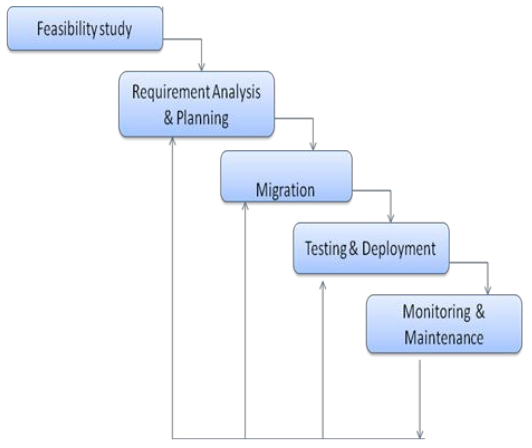
\includegraphics[width=\textwidth]{images/fuenf-phasen-wasserfall-modell.png}
\caption{Das Fünf-Phasen-Wasserfallmodell aus \protect\citeflow{fivephases} }
\label{fuenf-phasen-wasserfall-modell}
\end{center}
\end{figure}
\begin{description}
	\item[Phase 1 - Machbarkeitsstudie] In dieser Phase wird ergebnisoffen
geprüft, ob die Migration einer Anwendung technisch und wirtschaftlich möglich
und sinnvoll ist. Dabei wird nicht nur die Anwendung selbst analysiert, sondern
auch alle Rahmenbedingungen, die Einfluss auf das Verhalten des Systems ausüben
können. Außerdem wird eine detaillierte Kosten-Nutzen-Analyse erstellt.

	\item[Phase 2 - Anforderungsanalyse und -Planung] Um die zu migrierende
Anwendung und ihre Anforderungen zu verstehen, wird in der Planungsphase die
bestehende IT-Umgebung unter Berücksichtigung der genannten, die Migration
beeinflussenden Faktoren (siehe  Kapitel
\ref{cha:migration_bestimmende_faktoren})
genau begutachtet. Gilt die Anwendung auch nach Begutachtung als zur Migration
geeignet, werden der Return on Investment (ROI) sowie die Total Cost of
Ownership (TCO) berechnet, um die durch die Migration entstehende
Kostenvorteile
zu verstehen.

	\item[Phase 3 - Migration] Die existierende Anwendung wird in die Cloud
portiert und in Hinblick auf Leistungsfähigkeit und Performanz strukturiert
getestet. Zum Schluss wird die neue Plattform in einem User Acceptance Testing
(UAT) validiert.

	\item[Phase 4 - Tests und Auslieferung] Die Daten aus der Produktion
werden in die Cloud portiert. Anschließend wird die Software erneut getestet
und freigegeben. In dieser Phase ist ein hoher Grade an Überwachung und Support
nötig, um unvorhergesehene Probleme auffangen zu können. Unter Umständen wird
parallel zum Start der Cloud-Anwendung die Altsoftware zunächst weiter
betrieben.

	\item[Phase 5 - Überwachung und Wartung] Nach der Migration in die
Cloud ist es naturgemäß notwendig, die Leistungserfüllung durch den Anbieter in
Hinblick auf Leistungsfähigkeit, Verfügbarkeit und Sicherheit zu überwachen um
gegebenenfalls Gegenmaßnahmen einleiten zu können.
\end{description}


\subsection{TODO: Hinweis, dass sich diese Arbeit auf die ersten drei Phasen
beschränkt}

\begin{comment}

\subsection{Cloud-Computing}
Da die Definition von "`Cloud-Computing"' des National Institute of Standards
and Technology (NIST) \pcite{}{}{NIST} in \citeflow{thoughtsOnCloud} als gute
Grundlage geschätzt wird und auch in \citeflow{fivephases}, in dem das
Fünf-Phasen-Modell vorgestellt wird, als Basis dient, übernehme ich die
Definition in übersetzter Form aus \citeflow{softwareindustrie2015}:
\begin{cloudcomputing}
"`Ein Modell, das einen komfortablen, bedarfsabhängigen und netzbasierten
Zugriff auf eine gemeinsam benutzte Menge konfigurierbarer Rechenressourcen
ermöglicht, die schnell, mit geringem Verwaltungsaufwand und ohne (menschliche)
Interaktion mit einem Anbieter bereitgestellt und wieder freigegeben werden
können."'
\end{cloudcomputing}
Laut NIST besteht die "`Cloud"' als Modell neben fünf Charakteristika und drei
Service Modellen aus vier Einsatzmodellen (im Englischen: "`Deployment
Models"'). Da sie für das Verständnis des Fünf-Phasen-Modells nebensächlich
sind, wird hier nur kurz auf die Einsatzmodelle eingegangen. In ihnen geht es
darum, ob die Cloud ausschließlich von einer Organisation, von einer bestimmten
Gruppe von Organisationen oder von der Öffentlichkeit genutzt wird, wobei auch
Mischformen als Möglichkeit genannt werden. \pcite{}{}{NIST}

\subsubsection{Charakteristika}
Die fünf Charakteristika von Cloud-Computing, die in \citeflow{NIST} genannt
werden, lauten zusammengefasst:

\begin{description}
	\item[Selbstbedienung bei Bedarf:] Ein Nutzer kann ohne
zwischenmenschliche Interaktion mit dem Dienstleister die automatische
Zuteilung von Rechenkapazitäten anstoßen.
	\item[Umfassender Zugriff über das Netzwerk:] Die Dienstleistung ist
über das Netzwerk mit verschiedensten Geräten auf standardisierte Art und Weise
abrufbar, zum Beispiel mit einem Internet Browser.
	\item[Geteilte Ressourcen] Kunden eines Cloud-Anbieters teilen
sich physische oder virtuelle Rechenleistung, die dynamisch und bedarfsgerecht
zugeteilt wird. Im Allgemeinen hat der Nutzer weder Kenntnis noch
Kontrolle über den Ort der Speicherung und Verarbeitung seiner Daten. Abhängig
vom Anbieter lassen sich Orte aber vertraglich festlegen.
	\item[Schnelle Anpassungsfähigkeit] Rechenkapazitäten können dem Bedarf
entsprechend, teilweise automatisch, schnell zugewiesen und entzogen werden.
Auf den Kunden wirkt die abrufbare Rechenleistung oftmals unbegrenzt.
	\item[Vermessene Dienstleistung] Cloud Systeme messen und optimieren
Ressourcennutzung automatisch und stellen die Auslastung und die Nutzung sowohl
dem Cloud Anbieter als auch dem Nutzer zur Verfügung, da sie
Berechnungsgrundlage für die Kosten sind.
\end{description}

\subsubsection{Service Modelle - XaaS}
Service Modelle beschreiben, welche Leistungen "`as a Service"' angeboten
werden. Es gibt recht viele dieser Modelle - \citeflow{xAsAService} zählt 35
Varianten - die mehr oder weniger verbreitet sind und mit "`Everything as a
Service (XaaS)"' zusammengefasst werden. \pcite{}{95}{benlian_saas_2010} Nicht
zwangsläufig beschränkt er sich auf Technologien, die als Dienstleistung
angeboten werden. \pcite{}{872}{decision-making_in_cloud_computing_environments}
\\
\citeflow{NIST} sieht drei Service Modelle vor, die sich im Anteil der
selbst zu verwaltenden, technologischen Anteile (Integrationstiefe)
unterscheiden und in dieser
Hinsicht in Abbildung ~\ref{xaas_im_vergleich} mit der herkömmlichen IT
verglichen werden. Die Wahl des Modells wirkt sich auf den
Migrationsprozess aus. \pcite{}{213}{Pahl2013}
\begin{figure}[hb]
\begin{center}
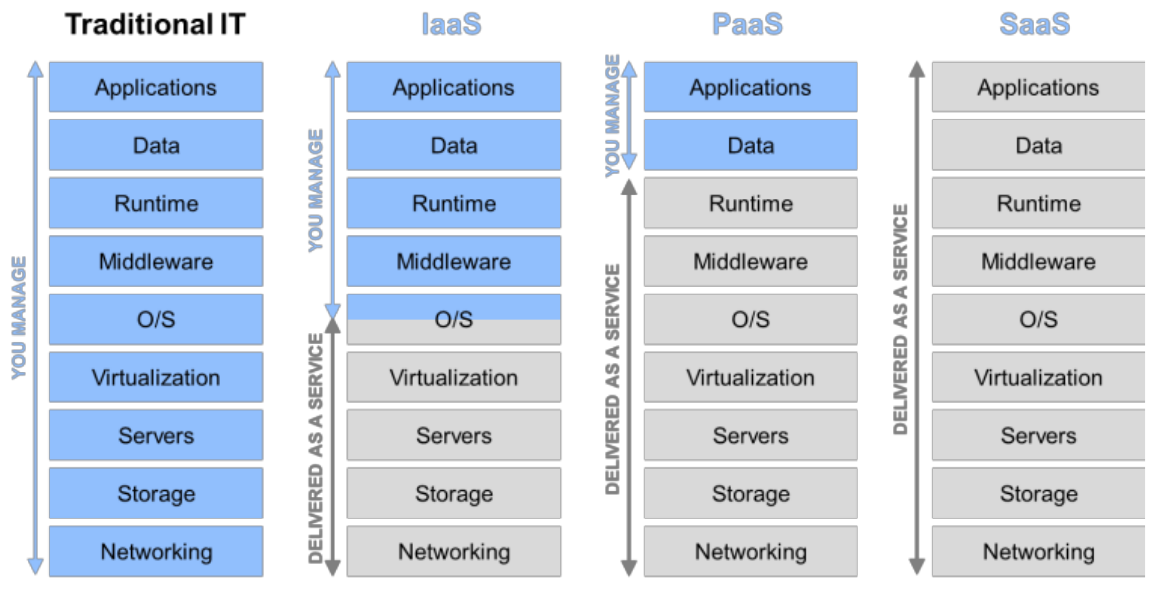
\includegraphics[width=\textwidth]{images/XaaS_im_Vergleich.png}
\caption{XaaS im Vergleich: Umfang von
Dienstleistung und Eigenverantwortung. Aus
\protect\citeflow{economics_of_the_cloud} }
\label{xaas_im_vergleich}
\end{center}
\end{figure}
\begin{description}
	\item[Infrastructure as a Service (IaaS)] Dem Kunden werden Netzwerk,
Speicher und Rechenleistung zur Verfügung gestellt. Über die darauf laufende
Software, teilweise sogar über das Betriebssystem kann selbst verfügt werden. \\
Kunden versprechen sich von IaaS vor allem Flexibilität in der Bereitstellung
und dem Betrieb von Servern, Datenspeichern und Netzwerkressourcen.
\pcite{}{213}{Pahl2013}
	\item[Platform as a Service (PaaS)] Der Kunde kann bereitgestellte
oder selbst entwickelte Software in der Cloud laufen lassen und eventuell
Einfluss auf die Anwendungsumgebung nehmen. \\
	\item[Software as a Service (SaaS)] Der Kunde kann eine vom Anbieter
bereitgestellte Software nutzen und in begrenztem Maße konfigurieren.
\end{description}



\subsecti
Als "`Cloud-Migration"' lässt sich der Begriff als  Diese Bereitstellung in der
Cloud ist zwar unter Umständen
mit keinen oder wenigen Änderungen zu erreichen, sollen aber Vorteile wie
Skalierbarkeit, Kosteneffizienz und Leistung erreicht werden,


Damit ist eine
Cloud-Migration viel mehr als eine Weiterentwicklung.
\pcite{}{}{framework_for_architecture-driven_migration}on{Migrationsformen}


\subsection{Salesforce}

\subsection{Anforderungen eines Independent Software Vendors (ISV)}



\subsection{Ideen}
\begin{description}
	\item[Migration] Sicht eines Unternehmens, das seine
On-Promise-Software in die Cloud schiebt versus ISV
\end{description}


\begin{comment}

\subsection{Herausforderungen in Migrationsprojekten als zu berücksichtigende
Faktoren}
Um die Eignung einer Anwendung für eine Migration in die Cloud zu prüfen,
schlagen \pcite{}{}{fivephases} die Berücksichtigung der folgenden der
folgenden wirtschaftlichen und technischen Faktoren vor. Um diese Faktoren in
einem geordneten Prozess zu berücksichtigen, führen sie ein Vorgehensmodell
ein. Dieses Vorgehensmodell hat den Vorteil, dass es an bestehende Strukturen
und Begrifflichkeiten anknüpft und sich deshalb besonders gut vergleichen,
ergänzen und diskutieren lässt. Aus diesem Grund soll es den Rahmen dieser
Arbeit bilden.

\subsubsection{Wirtschaftliche Faktoren}

\subsubsection{Technische Faktoren}




\subsubsection{Organisationsform als Einflussfaktor}
\citeflow{fivephases} identifizieren die Organisationsstruktur, beziehungsweise
deren Größe und Komplexität und insbesondere drei Formen als
wesentliche Einflussfaktoren für dieses Vorgehensmodell. Zu diesem Ergebnis
kommen auch \citeflow{Pahl2013}.
\begin{description}
	\item[Große Unternehmen] haben gewachsene, komplexe IT-Strukturen, die
umso detailliertere Analysen der Cloud-Eignung einzelner Anwendungen
erforderlich machen und eine Schrittweise Migration nahelegen, bei der
zunächst einfache Standardanwendungen wie E-Mail-Anwendungen migriert werden.
Komplexe Anwendungen folgen sobald Erfahrungen im Cloud-Umfeld gesammelt wurden
und gegebenenfalls fertige Anwendungen in der Cloud bereits existieren.
	\item[Kleinere und mittlere Unternehmen] haben gegenüber großen
Unternehmen nicht nur den Vorteil einer kleineren, weniger komplexen
IT-Landschaft. Bestehende Unternehmensprozesse lassen sich auch leichter an die
Cloud-Nutzung anpassen, sodass sich viele bereits in der Cloud existierende
Cloud-Anwendungen als SaaS nutzen lassen. Durch die nutzungsabhängige
Bepreisung lassen sich in der Cloud möglicherweise Anwendungen nutzen, die
bisher zu teuer oder zu komplex waren. Die nutzungsabhängige Bezahlung birgt
allerdings wie bereits geschildert auch Risiken, die neben den anderen Faktoren
ebenfalls vor der Migrationsentscheidung berücksichtigt werden sollten.
	\item[Regierungsorganisationen] dürften regelmäßig zwei Spezifika
aufweisen, die bei der Prüfung der Cloud-Eignung einer Anwendung zu prüfen
sind. Erstens sind sie in besonderem Maße, teilweise durch Gesetze, zur
Kontrolle über die eigenen Daten und Funktionsfähigkeit ihrer Anwendungen
gezwungen. Zweitens übersteigt die orts-, amts- oder ministerienübergreifende
Zusammenarbeit die Komplexität von großen Unternehmen bei weitem.
\end{description}



\subsection{Methoden zur Anforderungsermittlung in Migrationsprojekten}
\subsection{Aktuelle und prognostizierte Ressourcennutzung}
\subsection{Auswahl des Migrationsziels in der Cloud}
\subsection{Kostenabschätzung der Cloud-Lösung}

\newpage
\subsection{Abbildungen}

\begin{figure}[h]
\begin{center}

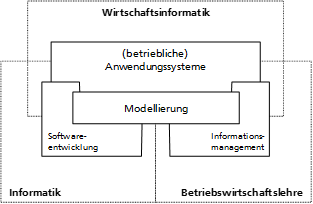
\includegraphics[width=10cm]{images/Abb2_3.png}
\caption{Einordnung der Wirtschaftsinformatik (angelehnt an Fink et al. 2001)}
\label{Abbildung2_3}
\end{center}
\end{figure}
Bitte achten Sie darauf, dass alle vorhandenen Abbildungen und Tabellen in einem inhaltlichen Zusammenhang mit dem Text stehen und Sie auf die entsprechende Abbildung (bspw. Abbildung 1) verweisen.
\subsection{Tabellen}
%hier Tabelle einfügen
\begin{table}[h]
\centering
\begin{tabular}{ccc}
\hline \textbf{Attribute} &\textbf{Typ}  & \textbf{1. Ausprägung (Beispiel)} \\
\hline Titel & \textit{STRING}& Aktiengesetz (AktG)  \\
Text& \textit{STRING} &  [Text des AktG]\\
Gültig von & \textit{DATE} & 01.01.2010 \\
Gültig bis & \textit{DATE} & - \\
Dok.-Besitzer & \textit{STRING} & Rechtsabteilung \\
Quelle & \textit{STRING}  & Deutsche Gesetze \\
Verplichtungsgrad & \textit{STRING} & verplichtend \\
\hline
\end{tabular}
\caption{Attribute der Anforderungsquellen im Metamodell}
\label{tab:tabelle 1}
\end{table}
\par\medskip

Tabelle 1 stellt eine beispielhafte Tabelle dar
\end{comment}
